% !TEX TS-program = pdflatexmk

% Style for a MSc paper at Warsaw School of Economics
% Michał Ramsza
% Friday, December 14, 2012

% --- document class and other global stuff ---------------------------
\documentclass[english, twoside, 12pt, a4paper]{article}

% --- packages --------------------------------------------------------
\usepackage{textcomp}
\usepackage{times}
\usepackage{amsmath}
\usepackage{amsfonts}
\usepackage{amssymb}
\usepackage{amsthm}
\usepackage[T1]{fontenc}
\usepackage[utf8]{inputenc}
\usepackage{graphicx}
\usepackage{xcolor}
\usepackage{enumitem}
\usepackage[english]{babel}
\usepackage[centering, left=3.5cm, right=2.5cm, textheight=24cm]{geometry}
\usepackage{listings}
\usepackage[]{algorithm2e}

% --- packages for citations ------------------------------------------
\usepackage{natbib}
\AtBeginDocument{\renewcommand{\harvardand}{and}}

% --- package for automatic insertion of R code -----------------------
\usepackage{listings}
\lstset{%
   numbers=left,%
   tabsize=3,%
   numberstyle=\footnotesize,%
   basicstyle=\ttfamily \footnotesize \color{black},%
   escapeinside={(*@}{@*)}}

%\lstset{language=R,%
%   numbers=left,%
%   tabsize=3,%
%   numberstyle=\footnotesize,%
%   basicstyle=\ttfamily \footnotesize \color{black},%
%   escapeinside={(*@}{@*)}}


% --- support for links -----------------------------------------------	
\usepackage{url}
\usepackage{hyperref}
\hypersetup{colorlinks=true,
            linkcolor=black,
            citecolor=darkgray,
            urlcolor=darkgray,
            pagecolor=darkgray}

% --- support for large tables and other stuff ------------------------	
\usepackage{longtable}
%\usepackage{subfigure} % this package will not work with subcaption package
\usepackage{float}
\usepackage{caption}
\usepackage{subcaption}
\usepackage{wrapfig}
\usepackage{pdflscape} % relevant for wide tables (rotating pages)

% --- support for game theory ------------------------------------------
\usepackage{sgame}

% --- support for no widows --------------------------------------------
\usepackage[defaultlines=4,all]{nowidow}

% --- quotation for polish language \enquote{}
\usepackage[autostyle]{csquotes}
\DeclareQuoteAlias{dutch}{polish}

% --- definitions for environments -------------------------------------
\theoremstyle{definition}
    \newtheorem{condition}{Assumption}
    \newtheorem{example}{Example}      

\theoremstyle{plain}
    \newtheorem{definition}{Definition}    
    \newtheorem{proposition}{Proposition}
    \newtheorem{theorem}{Theorem}
    \newtheorem{cor}{Corollary}

\theoremstyle{remark}
    \newtheorem{remark}{Remark}

% --- other settings --------------------------------------------------
\linespread{1.5}
\frenchspacing
\sloppy
\allowdisplaybreaks[4]
\raggedbottom
\clubpenalty=10000
\widowpenalty=10000

% --- only if required ------------------------------------------------
\AtBeginDocument{\renewcommand*{\figurename}{Figure}}
\AtBeginDocument{\renewcommand*{\tablename}{Table}}

% --- changing definition of footnote ---------------------------------
\makeatletter
\renewcommand\footnotesize{%
   \@setfontsize\footnotesize\@ixpt{10}%
   \abovedisplayskip 8\p@ \@plus2\p@ \@minus4\p@
   \abovedisplayshortskip \z@ \@plus\p@
   \belowdisplayshortskip 4\p@ \@plus2\p@ \@minus2\p@
   \def\@listi{\leftmargin\leftmargini
               \topsep 4\p@ \@plus2\p@ \@minus2\p@
               \parsep 2\p@ \@plus\p@ \@minus\p@
               \itemsep \parsep}%
   \belowdisplayskip \abovedisplayskip
}
\makeatother

\newcommand{\todo}[1]{\noindent{\color{red}>>~#1}}

\newcommand{\setn}{\mathbb{N}}

% ---------------------------------------------------------------------
\begin{document}

% --- strona tytulowa -------------------------------------------------
\begin{titlepage}
\centering


\includegraphics[width=0.66\textwidth]{logo.JPG}

\vspace*{0.5cm}
Studium licencjackie\\
\begin{flushleft}
Kierunek: Metody Ilościowe w Ekonomii i Systemy Informacyjne\\
%Specjalność: <specjalność> % w przypadku braku należy pominać
Forma studiów: Stacjonarne
\end{flushleft}

\vspace*{.5cm}
\rule{0cm}{1cm}\hfill
\begin{minipage}{9cm}
Imie i nazwisko autora: Kacper Mordarski\\
Nr albumu: 101247
\end{minipage}

\vspace*{1cm}
\begin{minipage}{12cm}
\centering
\Large
\textbf{Cooperation in the PD and SD games\\on preferential attachment graphs}
\end{minipage}

\vspace*{2cm}
\rule{0cm}{1cm}\hfill
\begin{minipage}{9cm}
Praca licencjacka napisana\\
w Katedrze Matematyki i Ekonomii Matematycznej\\
pod kierunkiem naukowym\\
dr hab. Michała Ramszy
\end{minipage}

\vfill
Warszawa 2022
\end{titlepage}

\rule{1ex}{0ex}\clearpage

% --- table of contents -----------------------------------------------
\cleardoublepage
\tableofcontents

% --- chapter ---------------------------------------------------------
\cleardoublepage
\section{Introduction}

This paper aims to replicate, to some degree, the seminal paper of \cite{santos2005scale} on the emergence of cooperation. The secondary goal of this research is to provide the publicly available code allowing replication of the actual results.
 
The paper in question was published in \enquote{Physical Review Letters} on the 26th of August 2005 and, according to Google Scholar, has been cited over 1600 times since. It clearly shows the magnitude of the said paper and its groundbreaking character. The said paper presents the results of simulations conducted by the authors and their implications for evolutionary game theory.
 
The crucial thing to note is that the authors of the said paper changed the approach to modeling cooperation in games on networks by using the Scale-Free Networks (SFN). At that time, it was standard to use regular networks to model connections between players. Scale-Free Networks are characterized by a completely different degree distribution that follows the power law. Such networks are usually the results of a growth governed by the preferential attachment rule. 

When we analyze some real networks, for example, the Twitter network, we observe that users with a larger number of \enquote{followers} are more likely to gain new ones than accounts with a low number of \enquote{followers}. The fundamental assumption is that the networks of contacts in societies have the same characteristic. 
 
One of the goals of \cite{santos2005scale} was to compare the results of simulations on different kinds of graphs. According to their results, players that occupy vertices of SFN are much more likely to cooperate than on some other type of graph. Those results came up in the Snowdrift game (later referred to as SD) and Prisoners Dilemma game (later referred to as PD).  

Our work consists of several sections describing concepts and methods necessary to conduct simulations and therefore replicate results presented in \cite{santos2005scale}. We started off by presenting mathematical and economic ideas used later on. 

In section~\ref{sec:gt}, we introduce elements of noncooperative game theory crucial for understanding the underlying mechanisms of our work, e.g., the Nash equilibrium or the normal-form game. Those concepts are being established in a way as simple as possible to make the text easy to follow and comprehend. We also provide simple examples of games (\enquote{Battle of sexes}, \enquote{Stag hunt}), and include an analysis of said games.

Section~\ref{sec:graphtheory} is on the topic of the graph theory. Since the structures of connections between players are modeled on the scale-free networks, we begin with a gentle introduction of basic concepts --- a definition of a graph, vertices, and edges. Then, we move to more sophisticated ideas and characteristics --- degree distribution, the procedure of creating the scale-free networks. We visualize the described graphs on figures~\ref{fig:graphsa}--\ref{fig:graphsc}.

The fourth chapter applies the concepts introduced in section~\ref{sec:gt} to games that are the foundation for our simulations (e.g., PD and SD). We describe those games, analyze their equilibria for different payoff parameters, and conclude the interpretation in terms of population games. In this section, we also introduce the idea of playing games on graphs representing the population of players. For the description to be complete, we also bring in the concept of learning in such games.

Section~\ref{sec:alg} is arguably the most important one because we describe our understanding of algorithms and mechanisms introduced in \cite{santos2005scale}, as well as presenting our implementation of said algorithms in the form of pseudocode. To be precise, we present in this chapter the description of the algorithm concluded from \cite{santos2005scale}, highlighting functions that had to be defined by us. Finally, we present the pseudocode implementation of all concepts and ideas that have been presented so far in this paper.

The second to last chapter includes the results generated by our algorithms. We present figures, laying out our results in a form that's comparable with those in \cite{santos2005scale} --- our final results are presented as plots of averaged cooperation/defection proportions for given parameters of PD and SD. We also describe the data manipulation necessary to obtain such results, so that they can be easly replicated. 

In the last section, we conclude the discussion on the results and methods used to obtain them. There are also included ideas for further development of our study and the direction in which we would like to lead them. 

The entirety of the code used to perform steps described throughout this paper are to be found on GitHub: 
\url{https://github.com/kMordarski/Thesis}.

% --- chapter ---------------------------------------------------------
\clearpage
\section{Elements of the noncooperative game theory}\label{sec:gt}

The current chapter introduces the most fundamental concepts in the game theory and the appropriate notation. These concepts and notation are used later in subsequent chapters. The exposition follows \cite{fudenberg1991game,gibbons1992game}.

\subsection{Normal-form game}

The noncooperative game theory is the basis for this paper. We call a game a noncooperative game if all of the game's participants (players) act in their own best interest and, therefore, compete with each other. Moreover, they need to be rational --- choose a strategy based on its optimality. Games in this paper are presented as normal-form games. The definition of a norm-form game requires a couple of elements. 

First of all, let us define a set of players $i \in I$, where $I$ is a finite set of natural numbers, i. e., $I = \{1, 2, \ldots, N\}$. For each player $i$, we define the pure strategy space $S_i$ consisting of $k_i \in \setn$ pure strategies. The sequence of pure strategies $s = \left(s_1, \ldots, s_N \right) \in \prod_{i \in I} S_i = S$ is called the strategy profile. Lastly, we define a payoff functions, denoted as $u_i(s)$. A function \(u_i (s)\) maps a strategy profile \(s\) into player's payoff, that is $u_i: \prod_{i \in I}S_i \rightarrow \mathbb{R}$.

The last two assumptions of a normal-form game are that (a) players act independently and (b) the perfect knowledge is assumed. The former assumption means that players have no knowledge of other players' choices while making a decision. The latter means, roughly, that all players know the structure of the game and it is perfect knowledge.

\subsection{The Nash equilibrium}

The fundamental concept of the game theory is the concept of equilibrium. The most widely used and accepted concept of equilibrium is Nash equilibrium, cf.~\cite{nash1951non}. The general idea of the Nash equilibrium concept is that there is a strategy profile in which none of the players have an incentive to alter their strategy. Given a profile of strategies \(s\), no single player can change a strategy to get a higher payoff.

Technically, we define the Nash equilibrium as follows. Let $S_i$ be be the set of all possible strategies for a player $i$, and let $s^* = (s^*_i, s_{-i}^*)$ be a strategy profile, where $s_{-1}^*$ denotes strategies of all other players except of $i$. For the strategy profile $s^*$ to be the (weak) Nash equilibrium, it must satisfy the inequality:
\[
\forall s_i \in S_i:\:u_i(s_i^*, s_{-i}^*) \geq u_i(s_i, s_{-i}^*).
\]
For the Nash equilibrium to be strict, it must satisfy the strict inequality:
\[
\forall s_i \in S_i:\:u_i(s_i^*, s_{-i}^*) > u_i(s_i, s_{-i}^*).
\]

It is important to note that obtaining a Nash equilibrium does not guarantee the solution's optimality. To be specific, it means that payoffs may not be Pareto optimal \citep{wozny2012lecture}. Thus, there may exist a strategy profile yielding higher payoffs for at least one player with other players' payoffs not lower.

\subsection{Example games}

We conclude this chapter with two simple examples of normal-form games and their Nash equilibria. We start with the \enquote{Battle of sexes} game. The game described in \cite{luce1989games} is a classical decision analysis problem. Let us consider two music critics. They agreed to attend one of the two excellent concerts happening in their whereabouts. They can either go to a Shostakovich or Stravinsky concert. 

One critic --- let us call him player one --- would prefer to go to the Shostakovich concert. Meanwhile, the other critic, let us call him player two, would instead attend the Stravinsky concert. Unfortunately, they have no way of contacting each other, and therefore, the decision of where to go must be undertaken simultaneously.
We have two players, each with two possible strategies: \(\{Shostakovich, Stravinsky\}\). Each of them achieves a payoff of \(1\) if they get to go to their place of choice. Furthermore, if they both choose to go to the same event, they gain utility from spending time together. We can represent this game in form of the following payoff matrix:
\begin{center}
  \begin{game}{2}{2}
    & $Shostakovich$    & $Stravinsky$    \\
  $Shostakovich$ & $3,2$ & $1,1$  \\
  $Stravinsky$ & $0,0$ & $2,3$
  \end{game}
\end{center}
In the matrix, player one chooses the row strategy, and player two chooses the column strategy. Each cell represents two payoffs --- the left one is the first player's payoff, and the right one represents the second player's payoff. 

There are two Nash equilibriums in this game. They occur for the following strategy profiles: \((Shostakovich, Shostakovich)\) and \((Stravinsky, Stravinsky) \).

The second example concerns the \enquote{Stag Hunt} game. The stag hunt game originates from the work of Jean-Jacques Rousseau, cf.~\cite{rousseau1985discourse}. It represents the conflict between social cooperation and conflict. 

The idea behind the game is that two hunters can either hunt for a stag or a hare. Moreover, none of the hunters can single-handedly take down a stag --- it is a job for two. If either hunter chooses to go for a stag and the other selects a hare, they get payoffs equal to \(0\) and \(4\), respectively. If they both go for a hare, each gets a payoff of \(2\) --- there are only so many hares that they can provide an accumulated utility of 4. However, if they both decide to go for a stag, they get a payoff equal to \(5\). Therefore, the payoff matrix looks as follows:
\begin{center}
  \begin{game}{2}{2}
    & $Stag$    & $Hare$    \\
  $Stag$ & $5,5$ & $0,4$  \\
  $Hare$ & $4,0$ & $2,2$
  \end{game}
\end{center}

This game also has two Nash equilibriums --- strategy profiles \((Stag, Stag)\) and \((Hare, Hare)\). Clearly, the equilibrium \((Stag, Stag)\) is Pareto optimal. 

In the remaining of this paper, we only use two-player normal-form games without mixed strategies. Hence, the above introduction is sufficient for our purposes.

% --- chapter ---------------------------------------------------------
\clearpage
\section{Elements of the graph theory}\label{sec:graphtheory}

In this chapter, we focus on the topic of graph theory. We introduce the concepts essential for the description of mechanisms and procedures used in carrying out the simulations. 

\subsection{Non-directed graph}

The next important element that we use in the current paper is the graph theory. We can define a graph as two sets --- one containing objects called vertices and the other containing pairs of vertices called edges, cf.~\cite{ross1985discrete}. A single vertex is usually denoted by a natural number. It can stand for various objects, but in this paper, we use the vertices of a graph to represent players. The edges epitomize relations between vertices. In our case, the connected vertices stand for connected players. Thus, these players can engage in a game. We can distinguish between two types of a graph --- directed and undirected ones. As we use only undirected graphs, only these graphs are discussed below.

 \begin{figure}[hbt]
  \centering
  \begin{subfigure}[t]{0.40\textwidth}
    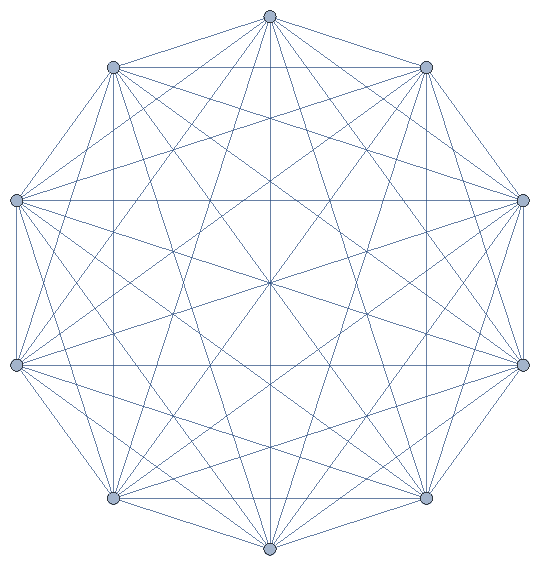
\includegraphics[width=\textwidth]{../ramsza/figs/graph_complete.pdf}
    \caption{Regular graph with \(n = 10\) vertices}
    \label{fig:graphsa}
  \end{subfigure}
  \hfill
  \begin{subfigure}[t]{0.40\textwidth}
    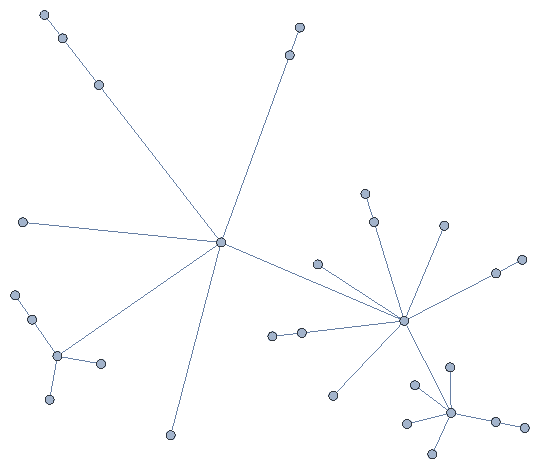
\includegraphics[width=\textwidth]{../ramsza/figs/graph_ba.pdf}
    \caption{BA graph with \( n = 30 \) and \( k = 1\)}
    \label{fig:graphsb}
  \end{subfigure}
  
    \begin{subfigure}[t]{0.40\textwidth}
    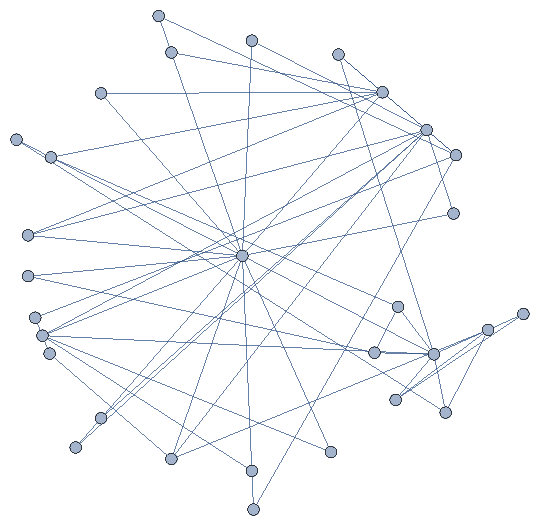
\includegraphics[width=\textwidth]{../ramsza/figs/graph_ba_a.pdf}
    \caption{BA graph with \( n = 30 \) and \( k = 2\)}
    \label{fig:graphsc}
  \end{subfigure}
  \hfill
  \begin{subfigure}[t]{0.40\textwidth}
    
\includegraphics[width=\textwidth]{../ramsza/figs/empty.pdf}
  \end{subfigure}
  
  \captionsetup{margin=10pt,font=small,labelfont=bf,width=.8\textwidth}

  \caption[Exampls of graphs]{Example of regular and BA graphs. \textit{Source:} own calculations}\label{fig:graphs}
\end{figure}

Since in an undirected graph edges represent relations with no regard to their direction, we can denote the relation between vertices $a$ and $b$ either as \(\{$a,b$\}\) or \(\{$b,a$\}\). As an example of an undirected graph, we can think of a graph in which vertices represent humans and edges represent relations between humans, e.g., being friends or connected in a given social network. 

Since these relationships work both ways (if subject \( a\) is a friend of subject \( b\), it implies that subject \(b\) is a friend of subject \(a\)), we only need to use a set \(\{a, b\}\) to denote an edge. We do not use directed graphs in this paper. Henceforth, as a graph, we refer to an undirected graph. 

\subsection{Vertex neighborhood and degree distribution}

Let us define a neighborhood of a vertex in a graph. The neighborhood of vertex $v$ in a graph $G$ is a set of vertices adjacent to the vertex $v$. We call two vertices adjacent when they are connected. The graph induced by a neighborhood of \( v \) is called a neighborhood graph. This concept is crucial for our work because it will allow us to identify all of the vertices able to engage in a game with a previously chosen player. 

The degree of a vertex $v$ is a number of all vertices connected to the $v$. The important characteristic of a graph is its' degree distribution. The degree distribution is the probability distribution of degrees in a graph. This characteristic varies throughout the different types of graphs. For a regular graph, it is a single value with the probability of 1 because, in a regular graph, all of the vertices have the same degree. Figure~\ref{fig:graphsa} show an example of a regular graph. 

\subsection{Scale-Free Networks}

In our work, we use a type of graph called Scale-Free Network. This type of graph is generated according to the Barabasi-Albert Model, cf.~\cite{albert2002statistical}. The scale-free networks are built in a sequence of steps. We start with a single vertex and, in each step, add a single vertex. The new vertex is connected to the previous vertices with the probability proportional to the vertices' degrees. More precisely, the probability of attaching a new vertex to an already existing vertex \(v\) is given as:
\[ 
p_v = \frac{k_v}{\sum_{j} k_j},
\]
where $k_v$ is a degree of vertex $v$ and $\sum_{j} k_j$ is a sum of degrees of all existing nodes (which, since our graph is an undirected graph, is equal to twice the amount of existing edges). 

\begin{wrapfigure}{r}{.5\textwidth}
\centering

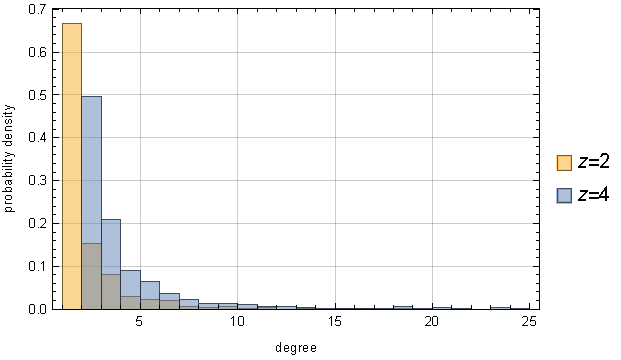
\includegraphics[width=.4\textwidth]{../ramsza/figs/dist.pdf}

\captionsetup{margin=10pt,font=small,labelfont=bf,width=.42\textwidth}

  \caption[Degree disribution]{Degree distribution in BA graphs. \textit{Source:} own calculations}\label{fig:dist}


\end{wrapfigure}

This rule favorites the vertices with higher connectivity and causes the graph to have so-called hubs. A hub is a term for a vertex with a considerably higher degree than other vertices. Thanks to this rule, the degree distribution of a graph follows the formula:
\[
P(k) \backsim k^{-3}.
\]
Figure~\ref{fig:dist} shows degree distributions in BA graphs for \(z = 2\) and \( z = 4\), where \(z\) is a double of average connectivity. Figures~\ref{fig:graphsb}--\ref{fig:graphsc} show example of scale-free networks. More precisely, figure~\ref{fig:graphsb} shows an example of a scale-free network built by adding only one edge at every step. Figure~\ref{fig:graphsc} show an example of a scale-free network created by adding two edges at every step. 




% --- chapter ---------------------------------------------------------
\clearpage
\section{Cooperation among the players}\label{sec:coop}

This chapter aims to apply the previously described game theory concepts to the cases used in the simulations. It means that we tell of the PD and SD games and then analyze them. We pay close attention to the parametrizations of the games and how they influence both their solutions (Nash equilibriums) and the eagerness to cooperate among the players.
We also introduce the concept of games played throughout the population of players on preferential attachment graphs and the learning mechanisms in such games. 

\subsection{A brief description of Snowdrift and Prisoners Dilemma games}

\paragraph{Prisoners Dilemma Game.} The Prisoners Dilemma game is a widely known problem in game theory and decision analysis. It shows situations in which the outcome is not optimal, even though players act in their own best interest. In the scope of our analysis, it is essential to note that in the PD game, the best strategy is to defect, regardless of the opponent's choice. The game is parameterized as follows:
\begin{center}
\begin{game}{2}{2}
  & $Cooperate$    & $Defect$    \\
$Cooperate$ & $R,R$ & $S,T$  \\
$Defect$ & $T,S$ & $P,P$
\end{game}
\end{center}
where the values are given as follows:
\[
\begin{aligned}
T &= b > 1, & R &= 1, \\
P &= 0, & S &= 0, \\
1 &< b \le 2. 
\end{aligned}
\]
We see that the above restrictions order the parameters as follows:
\[
T \geq R > P = S .
\]

\paragraph{Snowdrift Game.} The Snowdrift game represents a metaphor for cooperative interactions between players. Contrary to the PD game, the Snowdrift game stimulates cooperative behavior amongst players. It doesn't make the deflection strategy inapplicable, but the game's payoffs encourage cooperative behavior more than the payoffs of the PD game. The optimal strategy is to cooperate when the other defects and to defect when the other cooperates. The game is parametrized as follows:
\begin{center}
  \begin{game}{2}{2}
    & $Cooperate$    & $Defect$    \\
  $Cooperate$ & $R,R$ & $T,S$  \\
  $Defect$ & $S,T$ & $P,P$
  \end{game}
  \end{center}
where the parameters' values are:
\[
  \begin{aligned}
  T &= \beta > 1 , &  R &= \beta - \frac{1}{2} ,\\
  S &= \beta - 1 , &  P &= 0. 
  \end{aligned}
\]
We see that the above restrictions order the parameters as follows:
\[
 T > R > P > S .
\]

To represent the cost-to-benefit ratio of mutual cooperation we define $r$ as follows: 
\[
  r = \frac{1}{2\beta-1},
\] with $0<r\leq1$, cf.~\cite{santos2005scale}.

\subsection{Analysis of PD and SD games}

We use one-parameter parametrization for each of the PD and SD games. First, we discuss Nash equilibria in those games for the two extreme values of paramters \(b\) and \( r \). Let us start with a description of the Prisoners Dilemma game. For the smallest possible value of parameter $b$ equal to $1$, we represent the game as follows:
\begin{center}
  \begin{game}{2}{2}
    & $Cooperate$    & $Defect$    \\
  $Cooperate$ & $1,1$ & $0,1$  \\
  $Defect$ & $1,0$ & $0,0$
\end{game}
\end{center}
For the second case of PD we want to show the one with largest value of the parameter \( b \). The payoff matrix looks like the following:
\begin{center}
  \begin{game}{2}{2}
    & $Cooperate$    & $Defect$    \\
  $Cooperate$ & $1,1$ & $0,2$  \\
  $Defect$ & $2,0$ & $0,0$
\end{game}
\end{center}

For both of these cases, we obtain at least one Nash equilibrium. In the first case, we get two Nash equilibria. One for strategy profile $(Cooperate, Cooperate)$, the other for $(Defect, Defect)$. In both cases, the Nash equilibrium is weak, hence the players are indifferent to the choice of their strategy. In the case of $b = 2$, we have a single Nash equilibrium $(Defect, Defect)$. Moreover, in this case, the strategy $Defect$ is a weakly dominant strategy for both players. 

The term \enquote{strictly (weakly) dominant strategy} refers to a situation in which one of the player's strategies strictly (weakly) dominates any other strategy. Strategy \(a\) strictly dominates strategy \(b\) if the former yields higher payoffs regardless of the opponent's moves. The dominance is weak if the payoffs are not lower for all of the opponent's moves and higher for at least one, cf.~\cite{wozny2012lecture}. 

The parametrization of the SD games uses one parameter \( r \). To present the payoff matrix, we need to manipulate the formula:
\[
  r = \frac{1}{2\beta -1},
\] 
so that we can easily calculate the $\beta$ value. It's given as follows: 
\[
  \beta = \frac{1-r}{2r}.
\] 
The lowest value of $r$ is supposed to be as close to $0$ as possible. For this paper, we use the smallest value of $r$ equal to $10^{-5}$ and consider it a good enough approximation. For the said value of $r$, we write the payoff matrix as follows:
\begin{center}
  \begin{game}{2}{2}
    & $Cooperate$    & $Defect$    \\
  $Cooperate$ & $4999,4999$ & $4999.5,4998.5$  \\
  $Defect$ & $4998.5,4999.5$ & $0,0$
\end{game}
\end{center}
We conclude that, for this game, both players have a strictly dominant strategy $Cooperate$. Therefore, we also get a strict Nash equilibrium for the strategy profile of $(Cooperate, Cooperate)$. However, for \( r \rightarrow 0 \) we have \(\left| R / S\right| \rightarrow 1 \). Thus, the difference between the payoffs becomes less noticeable to players.

As the $r$ parameter reaches its highest\footnote{We use the highest value of \(r = 0.95\) in the subsequent simulations.} value $1$, the value of $\beta$ approaches to $0$. Thus, the payoff matrix looks as follows:
\begin{center}
  \begin{game}{2}{2}
    & $Cooperate$    & $Defect$    \\
  $Cooperate$ & $-\frac{1}{2},-\frac{1}{2}$ & $0,-1$  \\
  $Defect$ & $-1,0$ & $0,0$
\end{game}
\end{center}
The SD game with those payoffs also favorites the $Cooperate$ strategy because this strategy is dominant (even though it is only weakly dominant). There are, however, two Nash equilibria in this game. One occurs for the strategy profile of $(Cooperate, Cooperate)$, and the other is for strategy profile $(Defect, Defect)$. Even though the Nash equilibrium for $Defect$ gives higher payoffs, players are more likely to $Cooperate$ because of the strategy dominance.

% --- Gry na grafach losowych -----------------------------------------

\subsection{Games on graphs}

The model for the population of players in this paper is a previously described Barabasi-Albert model (i.e., Scale-Free Network). This model is generated randomly, with set parameters, for each simulation. Players occupy vertices of these graphs. Two players are able to engage in a game when they are connected --- there must exist an edge between two vertices. 

We use this type of graph because it is considered the best description of complex networks of agents in many areas of study --- e.g., biology, sociology, and economics \citep{volchenkov2002epidemic}. The most important characteristic of those graphs is that there exist \enquote{hubs} --- vertices with a considerably higher degree than the average. Those differences in vertices' degrees might be interpreted as inequalities among the players. 

\subsection{Learning procedure in population games}

The main objective of this paper is to present the proportion of $cooperate$ and $Defect$ strategies for both PD and SD games. To do so, we must introduce the concept of learning in population games. This idea is based on the hypothesis that players can \enquote{adapt} to the games' rules by changing their strategy. For the description of this procedure we rely on the \cite{santos2005scale}. 

The incentive for the players to alter their strategies is represented by their accumulated payoff. By the accumulated payoff, we mean the sum of all payoffs obtained by the player in the current generation. 
After all edges (pairs of connected players) engage in a single round of given game, one player is chosen arbitrarily --- let us call him player one. 

Then, from among all of his neighbors we randomly select one with a different strategy (i.e., if player one's strategy is $Cooperate$, we select a neighbor with a strategy $Defect$) --- let us name him player two.

We determine which strategy is to be altered. We do this by comparing their accumulated payoffs --- the player with a greater value will try to \enquote{take over} the other player and impose his strategy onto him. This procedure is nonetheless not definite and comes with a given probability. 

Let us introduce an example of player $1$ taking over player $2$. The probability of the transition is given as follows:
\begin{equation}\label{eq:pot}
  p_t = \frac{P_1 - P_2}{Dk_{>}},
\end{equation}
where $p_t$ is the probability of transition, $P_1$ and $P_2$ are accumulated payoffs of player one and player two, respectively. Parameter $D$ depends on the type of game that is being played --- generally speaking, it is the biggest obtainable payoff in a single round of a game, decreased by the $S$ or $P$ parameter for PD and SD, respectively. Therefore, for both PD and SD games, it is equal to the parameter $T$, because both $S$ and $P$ parameters are equal to $0$. The $k_{>}$ parameter is the greater value between both players' number of neighbors. If the transition is successful, we adjust the vector of strategies by altering the responding element. 

% --- chapter ---------------------------------------------------------
\clearpage
\section{Algorithms and simulations}\label{sec:alg}

This chapter contains a description of the functions, algorithms, and procedures used to conduct the necessary simulations. We must implement all mathematical concepts and ideas presented beforehand into a functioning code that allows us to produce analyzable results. The code is written in the Julia language to obtain high-efficiency code that is easy to follow and readable at the same time.

The description of the algorithm used in the paper~\cite{santos2005scale} is unclear. Thus, it is insufficient for exact replication. As a result, we may create a couple of different procedures based on different interpretations of said description. The algorithm described in this paper is the simplest and easiest to carry out among them. 

\subsection{Simulations description}

Because of the nature of this paper, our simulations must be conducted in strict accordance with the methods outlined
in \cite{santos2005scale}. Therefore it is only natural that we must follow each step with the utmost care and diligence. We must conduct 100 simulations for each parametrization. Each simulation is performed following those steps:
\begin{enumerate}[noitemsep]
  \item Setting up the parameters which are needed to create SF NOCs (such as the number of final vertices (population size), the average connectivity, etc.).
  \item Choosing the parameters, e. g. the payoffs, of the game which is to be simulated (either PD or SG).
  \item Creating the randomly generated SF NOC (we use the Barabasi-Albert model to do that). The SF NOC must be created in compliance with preferential attachment and 
  growth rules.
  \item Randomly distributing strategies amongst the population. Each vertex (player) can either get a $Cooperate$ or $Defect$ strategy.
  \item Every edge (i. e. two connected players) engages in a round of a given game --- this procedure is one \enquote{generation}. One simulation consists of 2100 generations. After each generation, an attempt is made to alter a strategy of one of the players.
  \item We collect results (equilibrium frequencies of cooperators and defectors) by averaging over the last 100 generations.
\end{enumerate}

\subsection{Functions}

In order to perform necessary calculations, it was necessary to define the following functions:

\begin{enumerate}
  \item \lstinline+Transform+ --- This function is used to map strategies onto a vector of arrays. As input, this function takes one of the edges of an SFN, as an output it returns a vector of length two (two vertices connected with an edge).
  \item \lstinline+Strat+ --- This function is used to map previously distributed strategies onto a vector of edges. As input, it takes an edge and as an output, it returns a vector of length two (two strategies previously attributed to the vertices).
  \item \lstinline+Games+ --- This function is used to evaluate the results of games played between players (vertices connected with an edge). As input, this function takes a vector of edges, a vector of strategies, and a vector of accumulated payoffs. It returns an adjusted vector of accumulated payoffs.
  \item \lstinline+CheckStrat+ --- This function fulfills a number of tasks. It takes as an input a randomly chosen vertex, vector of strategies, vector of accumulated payoffs, and the SFN. It identifies all neighbors of the previously mentioned vertex, then shuffles them, and then looks for a neighbor with a different strategy. Then it proceeds to change the strategy of the vertex with a lower accumulated payoff. The probability of the transition is described by equation~(\ref{eq:pot}).
\end{enumerate}

\subsection{Description of the algorithm}

The main algorithm is the fundamental element of this paper. It consists of 3 nested loops executing instructions necessary to conduct simulations, on which our research is based. These loops are described in the following part in an inside-out order. 

The first loop is responsible for evaluating the results of the games, potentially changing the strategies of players, and keeping track of the proportion of the strategies used by players. To run properly, it requires previously set parametrization and a set of edges of the Barabasi-Albert graph. As a result, it produces a vector of length \(100\) in which elements are the share of $Cooperation$ strategies, measured after each generation (\(2001\)--\(2100\)) in the population of players. This loop is repeated \(2000\) times, which gives us a total of \(2200000\) generations for one Barabasi-Albert graph parametrization for a given game.
The loop itself if given by the alogrithm~\ref{alg:loop1}.

\vspace*{1cm}
\begin{algorithm}[hbt]
  \KwData{Barabasi-Albert Model, array of edges, array of strategies, array of accumulated payoffs (initially equal to 0), empty vector of length 100, parametrization of the games}
  \KwResult{Vector of length 100 containing share of $Cooperation$ strategy for the population}
  initialization \;
  \For{k in generations}{

    \eIf{k is greater than $1$}{
      Adjust the array of strategies associated to players. \;
    }

    Play a single round of a given game between all possible pairs of players by applying function \lstinline+games+ on a vector of edges. \;
    Randomly choose one vertex.\;
    Attempt to change the strategy of the previously chosen player (or one of his neighbors) by applying function \lstinline+CheckStrat+. \;
   \eIf{k is greater than the number of generations minus $100$}{
    Evaluate the share of $Cooperate$ strategy in the entire population \;
    Save the result to the appropriate value of a vector. \;
    }{}
  }
\caption{The inner loop}\label{alg:loop1}
\end{algorithm}
 
\vspace*{1cm} 
 
The outer loop to the one described above is responsible for \enquote{resetting} the Barabasi-Albert graph. Since separate simulations are supposed to be carried out on a randomly generated SFN (but with the same parametrization), we need to conduct \(100\) of them (for each payoff parametrization); this loop is an indispensable element of the algorithm. The crucial fact to note is that this loop is also responsible for creating an object named \lstinline+ArrPath+ --- vector of length 100, used to store the results of the simulations. The procedure followed by this loop is given by the algorithm~\ref{alg:loop2}.

\begin{algorithm}[hbt]
  \KwData{Barabasi-Albert parametrization}
  \KwResult{Scale-Free Network built by Barabasi-Albert Model, list of edges, list of strategies, vector of accumulated payoffs, ArrPath --- an array of length 100 storing results of the simulations}
  initialization \;
  \For{j in simulations}{
   Create a Scale-Free Network by using the Barabasi-Albert model with previously set parameters.\;
   Create an array of length equal to the number of players, containing their strategies. \;
   Extract an array of edges from a previously created graph by mapping function \lstinline+transform+ onto a list of edges. \;
   Produce an array of tuples representing strategies for every player by mapping a function \lstinline+strat+ onto an array of edges. \;
   Create an array of accumulated payoffs (initially filled with zeros). \;
   Generate a vector of length 100 filled with zeros, called \lstinline+track+. This vector will be later on used to store the share of $Cooperation$ strategy. \;
   \eIf{j equals to 1}{
    Create an object called \lstinline+ArrPath+ with one element equal to \lstinline+track+. \;
    }{
    Merge the current \lstinline+track+ with \lstinline+ArrPath+. \;
   }
   Initiate the inner loop described above. \;
  }
  \caption{Second loop}\label{alg:loop2}
 \end{algorithm}

 The outer loop is in charge of setting the values of parameters of the games. Since we want to obtain \(20\) data points for a single Barabasi-Albert Model parametrization, we need to iterate 20 times executing the previously described loops. The payoffs for our games are in the range $[1,2)$ and $(0,1]$ for PD and SD, respectively. We need to divide the span (which is equal to 1 in both cases) by the number of data points, and we gain a result of \(0.05\). Thus, each iteration adds \(0.05\) to the payoffs of both games. Furthermore, this loop is also responsible for creating an object called \lstinline+DataToSave+ that stores our results. After the loop ends, the \lstinline+DataToSave+ object is saved into the local repository.
 
 \begin{algorithm}[hbt]
  \KwData{None}
  \KwResult{Parametrization for the games, \lstinline+DataToSave+ --- an array of vectors that will be used to store and ultimately save our results.}
  initialization\;
  \For{i in number of parametrizations}{
   \eIf{i is equal to 1}{
    Create an array of length 20 --- \lstinline+DataToSave+. ;
    }{
    Store the current \lstinline+ArrPath+ as a value of \lstinline+DataToSave+. \;
   }
   Set up payoffs of the games based on the current iteration. In each iteration, add 0.05 to the current values of the payoffs. \;
   Create a matrix of payoffs for the games with current parametrization. \;
   Initiate the second loop. \;
   Save \lstinline+DataToSave+ to the local repository. \;
  }
  \caption{The outer loop}
 \end{algorithm}
 
% --- chapter ---------------------------------------------------------
\clearpage
\section{Results and discussion}

In this chapter, we describe the data manipulations and methods used to transform our results into a readable and easy-to-present format. Then, we describe and discuss our results. We compare them to those presented in \cite{santos2005scale} and discuss the eventual discrepancies. 

\subsection{Format of obtained data}

The data we obtain is in form of a vector of length 20 --- let us call it $P$. Each value of this vector is another vector of length 100, containing vectors of length 100. Therefore it can be easily transformed into a vector of matrices of size $100 \times 100$. We interpret row number as a simulation's number (for each parametrization we performed 100 simulations) and column number as a generation's number from which the proportion is extracted. Therefore, we can present results for a single games' payoffs parametrization as follows:
\[
R = \begin{bmatrix} 
    r_{11} & \dots & r_{1M} \\
    \vdots & \ddots & \vdots \\
    r_{N1} &  \dots      & r_{NM} 
    \end{bmatrix}
,\]
where $R$ is a matrix of the results, $r_{NM}$ is the share of $Cooperate$ strategy after $2000 + M$ generations in the $N$-th simulation. Now, we may denote $P$ as:
\[
  P = (R_1, \dots, R_{20}),
\]
where $R_i$ is the matrix of results for the \(i\)-th iteration of the parametrization loop.

To present our data as a plot, we bring the $R_i$ matrices into a single value. We do that by simply averaging all matrix elements. The formula is as follows:
\[
  \frac{\sum_{k=1}^{N}\sum_{j=1}^{M} r_{kj}}{N \cdot M} .
\] 

Applying the above procedure to our vector \( P\) results in gaining 20 data points, and allows us to produce one plot for each Barabasi-Albert Model parametrization. Since we have three such parametrizations for each game, we gain 6 plots of the share of $Cooperate$ strategies. We've decided to group them in regard to games so that they could be easily compared. 

\subsection{Discussion}

The results we obtained seem to agree with the general intuition concerning the game theory. As we analyzed PD and SD games in section~\ref{sec:coop}, we highlighted the Nash equilibria and optimal, in this sense, strategies. For the PD game, we demonstrated that for the lowest value of the parameter $b$ (equal to \( 1\) ), players are indifferent to the choice of their strategies. 

% opis wyników dla PD

Figure~\ref{fig:resa} shows cooperation share profiles in the PD game. It is clear that for \(b\) close to \(1\) the share of cooperators is close to \(1/2\). This is quite clear, as for \(b \approx 1\) players are indifferent between strategies. As the value of $b$ increases, we can see that the average share of cooperators is decreasing. This is also a reasonable result --- $b$ parameter influences the dominance of $Defect$ strategy amongst the population of players. Thus, the higher the $b$ parameter is, the more competitive the $Defect$ strategy becomes. We may also observe that as the main Barabasi-Albert model's parameter --- average connectivity increases, the players tend to prioritize the dominant strategy more frequently. We can see it in Figure~~\ref{fig:resa} as profiles shift down. 

 \begin{figure}[hbt]
  \centering
  \begin{subfigure}[t]{0.45\textwidth}
    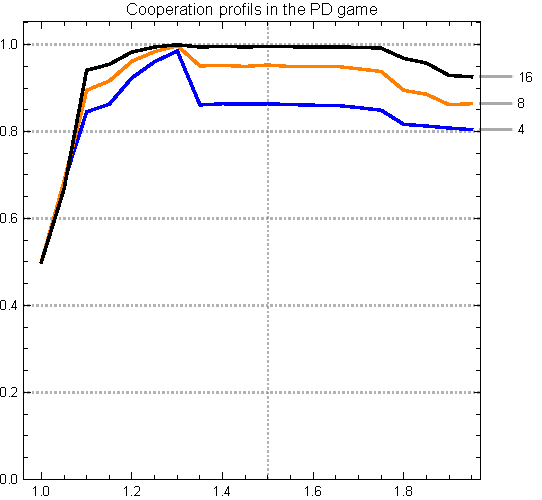
\includegraphics[width=\textwidth]{../ramsza/figs/PD_profiles.pdf}
    \caption{PD game}
    \label{fig:resa}
  \end{subfigure}
  \hfill
  \begin{subfigure}[t]{0.45\textwidth}
    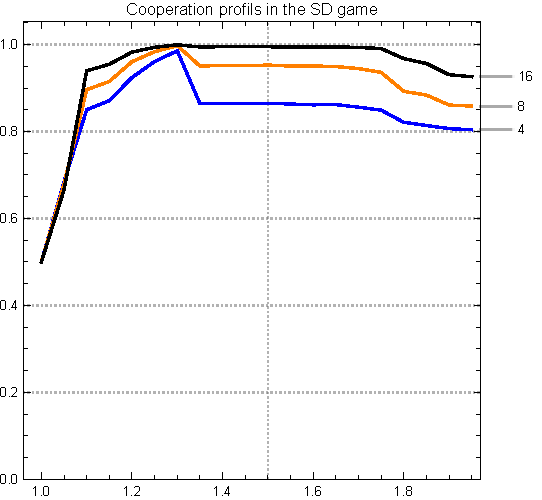
\includegraphics[width=\textwidth]{../ramsza/figs/SD_profiles.pdf}
    \caption{SD game}
    \label{fig:resb}
  \end{subfigure}

  
  \captionsetup{margin=10pt,font=small,labelfont=bf,width=.8\textwidth}

  \caption[Cooperation profiles]{Cooperation profiles for the PD and SD games. \textit{Source:} own calculations}\label{fig:res}
\end{figure}

% opis wyników dla SD

As far as the SD goes, we obtained the quite opposite results. Since the main parameter $r$ represents the cost-to-benefit ratio of mutual cooperation, we expect our curve to increase sharply for low values of \(r\) and then stay high, and only eventually start decreasing. We can see from the plot \ref{fig:resb}, that it is the case indeed. Moreover, we can conclude that with the increase in average connectivity, the share of $Cooperate$ strategy seems to react slower to the adjustments of $r$. This means that if players can engage in more games during each generation, they are more likely to change their strategies to $Cooperate$ even for a higher cost-to-benefit ratio. 

% porównanie do wyników oryginalnego paperu

Comparing our results to the results presented in the original paper~\cite{santos2005scale}, we must conclude, that our results differ. As far as the SD game is concerned, our results are similar for larger values of \(r\). For values \(r\approx 0\), our results are different and oscillate about \(1/2\). This seems to be intuitive since for such values relative ratio of payoffs is close to \(1\) and switching probabilities are, consequently,  close to \(1/2\). Thus, we conclude, that to a certain extent we have replicated the original results. 

As far as the PD game goes. Our results are more in line with the standard analysis of the PD game, that is, we do not observe a large cooperation share in the population. This is in stark difference from the original results. Obviously, we have to conclude that we have not replicated the original results. This may be because of two reasons. The first one is that the description of the algorithm in the original paper is vague. Consequently, we might have used the wrong or just a different algorithm. The second reason is, that the presented results might be wrong. 

% --- chapter ---------------------------------------------------------
\clearpage
\section{Conclussions}

% co zostało zrobione

Throughout the course of this paper, we have managed to accomplish --- to some extent, both of the goals set in the first chapter. We produced results that comply with the game theory intuition for the analyzed games. We also provided a replicable and easy-to-use code written in Julia language. 

% główny wynik

Those results do not, however, match completely the ones in \cite{santos2005scale}. Our main concern is that the high cooperation rate presented in the mentioned paper is neither obtainable with the procedure we used nor intuitive (since PD favorites defection strategy over the coop). Our procedure is of course debatable in terms of the number of conducted generations (we used $2100$ generations instead of $10100$). However, we can't think of any reason why increasing the number of generations would change the results so dramatically. The results for the SD game are, to some degree, similar to those obtained in the comparative article. It is only natural for the cooperation ratio to be high in a game that heavily favors the $Cooperate$ strategy.

% dalsze prace

We intend to explore other similar algorithms to further try to replicate the original results. Also, we will most certainly check the dependence of the results on the simulation lengths to assess the stability of the results.

\appendix
\section{Appendix: Julia code}

\lstinputlisting[]{../Julia/simulation.jl}


% --- bibliography ----------------------------------------------------
\clearpage
\bibliographystyle{agsm}
\bibliography{refs}

% --- abstract --------------------------------------------------------
%\clearpage
%\addcontentsline{toc}{section}{List of tables}
%\listoftables

% --- abstract --------------------------------------------------------
\clearpage
\addcontentsline{toc}{section}{List of figures}
\listoffigures

% --- abstract --------------------------------------------------------
\clearpage
\addcontentsline{toc}{section}{Streszczenie}
\section*{Streszczenie}

Podstawą tej pracy jest próba replikacji wyników oraz symulacji zawartych w pracy~\cite{santos2005scale}. Zawarliśmy w niej opisy wszelkich elementów niezbędnych do prawidłowego opisu
zjawisk oraz koncepcji będących podstawą wyżej wspomianych symulacji. 

Opisywane są zatem elementy teorii gier, takie jak profile strategii czy równowaga Nasha, jak również elementy teorii grafów --- definicje węzłów, krawędzi, czy opis rozkładów prawdopodobieństwa charakterystycznych dla danych grafów.

Następnie analizujemy gry PD oraz SD pod kątem elementów wymienionych w poprzedzających sekcjach, a także wprowadzamy pojecia gry rozgrywanej przez populację graczy reprezentowanej przy pomocy grafu oraz algorytmów uczenia się w grach populacyjnych. 

Kolejnym elementem naszej pracy jest przedstawienie implementacji algorytmów zastosowanych przez nas do replikacji wyżej wspomnianych wyników oraz ich reprezentacja w formie pseudokodu. W dwóch ostatnich rozdziałach demonstrujemy otrzymane wyniki oraz porównujemy je z tymi przedstawionymi w~\cite{santos2005scale}. Przedkładamy również naszą koncepcję na kontynuację rozpoczętych w tej pracy badań. 

Ostatnim elementem naszej pracy jest kod w jezyku Julia, pozwalający na replikację naszych wyników.
\end{document}


%%% Local Variables:
%%% mode: latex
%%% TeX-master: t
%%% End:
